\chapter{Definitionen und Erklärungen}

Bevor genauer in die Arbeit eingestiegenw erden kann, müssen jedoch erstmal die Ausgangsituation dargestellt, ein paar Begriffe geklärt und das Thema etwas abgesteckt werden.

\section{Projektbeschreibung}
Zu Beginn der Arbeit bestand bereits eine Website, die durch einen internen Workshop konzeptioniert und durch ein Pflichtpraktikum implementiert wurde. Die Website wurde mit der Web-Technologie Elixir gebaut, die sowohl Frontend als auch Backend beinhaltet. Hierbei handelt  es sich um eine Plattform, die das Ziel hat, das Verleihen und Leihen innerhalb von Bekanntschaftskreisen zu vereinfachen/ ermöglichen. Hierfür kann jeder Nutzer seine eigenen, verleihbaren Gegenstände auf der Plattform eintragen. Zusätzlich können Nutzer sogenannte Kreise erstellen und zusammen mit Freunden bzw. Familie beittreten. Jeder kann dann die Gegenstände sehen, die in den verschiedenen Kreisen verfügbar sind, in denen er Mitglied ist. Zur Kontaktaufnahme gibt es ein Chatsystem, bei dem sich Leute Nachrichten hin und her schicken können, um den Austausch zu organisieren.

\section{Funktionsumfang der Beispiel Anwendung}
Um mehrere Unterschiedliche Ansätze implementieren zu können, wurde die App, die entwickelt wurde, auf einen bestimmten Funktionsumfang beschränkt. Dieser soll dabei all das enthalten was bei einer typischen Appbenötigt wird. So hat man einfache Informationsseiten, einen Login, eine Authentifizierung, eine gewisse Art von Navigation, eine Listenansicht, eine Art permanente Speicherung von Daten für den Login und eine Kommunikation mit einem Server um Daten zu erhalten, schicken und evtl zu synchronisieren.

In Abbildung \ref{fig:pageflow} Kann man die in Android und Flutter implementierten Abläufe sehen.  

\begin{figure}[ht]
  \centering
  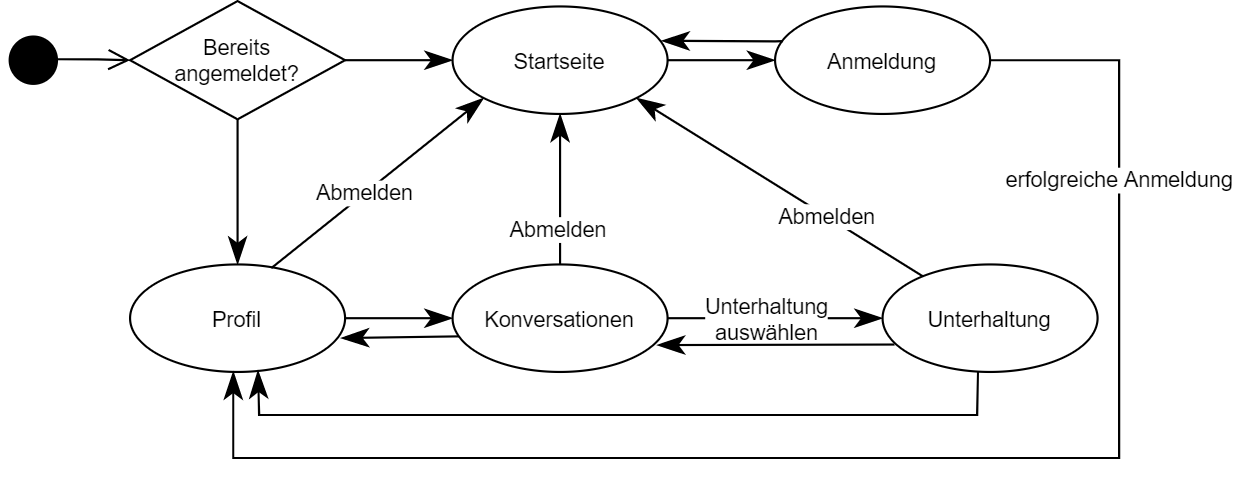
\includegraphics[height=7cm,keepaspectratio]{images/Pageflow_native_flutter.png} 
  \caption{Verbindungen zwischen den Seiten der implementierten Applikation }
  \label{fig:pageflow}
\end{figure}

\section{Themenabgrenzung}
Keine Spiele weil....
Kein iOS weil....


\section{Begriffe}
Wenn in dieser Arbeit von einer App bzw. Applikation geredet wird, so ist hiermit eine Anwendung gemeint, die für mobile Endgeräte, vorallem Smartphones mit den Betriebssystemen Android bzw. iOS gebaut wurden.
Außerdem ist in dieser Arbeit oft die Rede von Multi-Plattform-Anwendungen. Darunter versteht man eine Anwendung, die nicht nur für eine Plattform geschrieben wurde, sondern für mehrere. Das kann etwa die verschiedenen Smartphone Plattformen beinhalten, können aber auch die verschiedenen PC Plattformen mit einbegriffen werden. Eine Anwendung muss dabei auch nicht alle Plattformen beinhalten, sonder kann auch nur zwei Statt Multi-Plattform-Anwendungen wird häufig auch Cross-Plattform-Applikationen als Begriff genutzt, da dies ein in der Industrie häufig benutzter Wortlaut ist. 

\section{Die verschiedenen App Development Framework Klassen}
Wenn man über Applikationsentwicklung für mobile Endgeräte spricht, muss mann zwischen einigen verschiedenen Varianten unterscheiden.
\TODO{Muss auf jeden Fall noch Quellen, noch mehr und umschreiben.}
\subsection{Native Applikationen}
1.Native Apps:
Native Apps sind Applikationen die mit der Plattformspezifischen Programmiersprache für die einzelnen Plattformen entwickeltwerden. Hierbei wird dann in Kotlin für Android oder Swift für iOS sowohl die UI als auch die Logik der App umgesetzt und ist so gesehen ein eigenständiges System, da die dadurch entwickleten Applikationen nur auf der Plattform genutzt werden können, für die sie geschrieben wurden.
Oft verfügen diese Applikationen auch noch über externe Schnitstellen, oder einer Verbindung zu einem Server, um etwa auf Datenhaltung oder andere Dienste zuzugreifen.
Ein Vorteil dieser Art der Entwicklung ist es, dass man sehr gut die verschiedenen Möglichkeiten der jeweiligen Plattform ausnutzen kann. So ist etwa eine Nutzung der Kamera in nativ entwickelten Applikation deutlich einfacher und besser umsetzbar. Dazu kommt, dass man bessere Nutzeroberflächen bauen kann, die auf die mobile Plattform angepasst sind.
Der Nachteil den eine Native Entwicklung jedoch hat ist der Aufwand und die damit verbundenen Kosten. Um für die beiden vorherschenden Plattformen eine Applikation anbieten zu können, braucht man die doppelte Zeit, als wenn man nur eine App entwickelt. Kommt dann noch eine Website und Serveranwendung oder ähnliches hinzu, wird schnell aus einer kleinen Anwendung ein großer Kostenproduzent.
\subsection{Hybride Applikationen}
2. Hybride Apps:
Hybride Apps sind Applikationen die zu gewissen Anteilen aus nativem Code bestehen und zu gewissen Teilen Code, Schnitstellen oder Darstellungen anderer Websiten bzw. Webapplikationen nutzen. Der häufigste Anatz ist es hier, Webappplikationen zu einem gewissen Anteil in einem Frame der Applikation darzustellen und dabei einzelne Seiten durch nativ entwickelte Oberflächen zu ersetzen und die Daten an die Webapplikationen weiter zu geben. 

\subsection{Cross Plattform Applikationen}
3. Cross-Plattform-Apps
Unterscheidung zwischen Webview in App und z.B. Flutter 
